\section{Finding similar proteins: BLAST}
\subsection{Use the NCBI BLAST for creating a database of similar proteins. Use the non-redundant protein
sequences (nr) database and restrict the search to one species.}

I visited \href{https://blast.ncbi.nlm.nih.gov/Blast.cgi?PAGE=Proteins&PROGRAM=blastp&BLAST_PROGRAMS=blastp&PAGE_TYPE=BlastSearch&BLAST_SPEC=blast2seq&DATABASE=n/a&QUERY=&SUBJECTS=}{NCBI BLAST}, and uploaded the whole sequence (\texttt{Q62936.fasta}). After I searched database \textbf{Non-redundant protein sequences (nr)} using \textbf{Blastp (protein-protein BLAST)}, I restricted the search to species \textbf{Rattus Norvegicus}. The summary of the results are shown on Figure \ref{blastsum}.

\begin{figure}
\centering
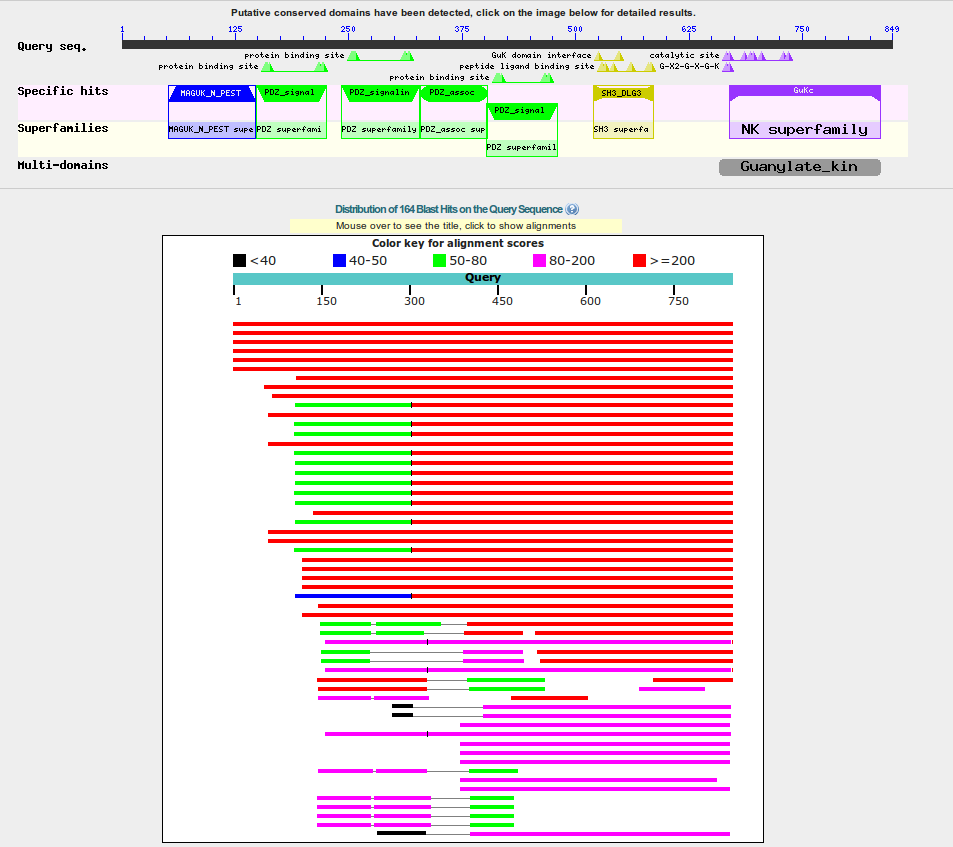
\includegraphics[width=\textwidth]{blast.png}
\caption{Result of searching database \textbf{Non-redundant protein sequences (nr)}}
\label{blastsum}
\end{figure}

As it can be seen, the search resulted in very high number of \emph{perfect} matches. This fact I would consider the hypothesis that the protein was evolutionary conserved over time, because its structure is replicated to many other similar proteins.
\paragraph{Choose 15-20 sequences from the same species BLAST hits. Shortly explain your choices.}
I chose the proteins listed in \url{~/files/ex5.fasta}, because they exhibit high level of \texttt{Query cover}, according to \href{https://blast.ncbi.nlm.nih.gov/Blast.cgi}{NCBI BLAST} and at the same time low level of actual identity.

\subsection{Create your database.}
I downloaded the proteins both in \texttt{complete} and \texttt{aligned} sequence. They can be found at: \url{~/files/ex5.fasta} and \url{~/files/ex5aligned.fasta}

\subsection{What kind of domains does blast find, are they the same as annotated in UniProtKB?}
I looked up the selected proteins on \emph{UniProtKB}, and found that the sites of match that can be seen on Figure \ref{blastsum}, are the sequences annotated in \emph{UniProtKB} as \textbf{PDZ} domains.